\documentclass[1p]{elsarticle_modified}
%\bibliographystyle{elsarticle-num}

%\usepackage[colorlinks]{hyperref}
%\usepackage{abbrmath_seonhwa} %\Abb, \Ascr, \Acal ,\Abf, \Afrak
\usepackage{amsfonts}
\usepackage{amssymb}
\usepackage{amsmath}
\usepackage{amsthm}
\usepackage{scalefnt}
\usepackage{amsbsy}
\usepackage{kotex}
\usepackage{caption}
\usepackage{subfig}
\usepackage{color}
\usepackage{graphicx}
\usepackage{xcolor} %% white, black, red, green, blue, cyan, magenta, yellow
\usepackage{float}
\usepackage{setspace}
\usepackage{hyperref}

\usepackage{tikz}
\usetikzlibrary{arrows}

\usepackage{multirow}
\usepackage{array} % fixed length table
\usepackage{hhline}

%%%%%%%%%%%%%%%%%%%%%
\makeatletter
\renewcommand*\env@matrix[1][\arraystretch]{%
	\edef\arraystretch{#1}%
	\hskip -\arraycolsep
	\let\@ifnextchar\new@ifnextchar
	\array{*\c@MaxMatrixCols c}}
\makeatother %https://tex.stackexchange.com/questions/14071/how-can-i-increase-the-line-spacing-in-a-matrix
%%%%%%%%%%%%%%%

\usepackage[normalem]{ulem}

\newcommand{\msout}[1]{\ifmmode\text{\sout{\ensuremath{#1}}}\else\sout{#1}\fi}
%SOURCE: \msout is \stkout macro in https://tex.stackexchange.com/questions/20609/strikeout-in-math-mode

\newcommand{\cancel}[1]{
	\ifmmode
	{\color{red}\msout{#1}}
	\else
	{\color{red}\sout{#1}}
	\fi
}

\newcommand{\add}[1]{
	{\color{blue}\uwave{#1}}
}

\newcommand{\replace}[2]{
	\ifmmode
	{\color{red}\msout{#1}}{\color{blue}\uwave{#2}}
	\else
	{\color{red}\sout{#1}}{\color{blue}\uwave{#2}}
	\fi
}

\newcommand{\Sol}{\mathcal{S}} %segment
\newcommand{\D}{D} %diagram
\newcommand{\A}{\mathcal{A}} %arc


%%%%%%%%%%%%%%%%%%%%%%%%%%%%%5 test

\def\sl{\operatorname{\textup{SL}}(2,\Cbb)}
\def\psl{\operatorname{\textup{PSL}}(2,\Cbb)}
\def\quan{\mkern 1mu \triangleright \mkern 1mu}

\theoremstyle{definition}
\newtheorem{thm}{Theorem}[section]
\newtheorem{prop}[thm]{Proposition}
\newtheorem{lem}[thm]{Lemma}
\newtheorem{ques}[thm]{Question}
\newtheorem{cor}[thm]{Corollary}
\newtheorem{defn}[thm]{Definition}
\newtheorem{exam}[thm]{Example}
\newtheorem{rmk}[thm]{Remark}
\newtheorem{alg}[thm]{Algorithm}

\newcommand{\I}{\sqrt{-1}}
\begin{document}

%\begin{frontmatter}
%
%\title{Boundary parabolic representations of knots up to 8 crossings}
%
%%% Group authors per affiliation:
%\author{Yunhi Cho} 
%\address{Department of Mathematics, University of Seoul, Seoul, Korea}
%\ead{yhcho@uos.ac.kr}
%
%
%\author{Seonhwa Kim} %\fnref{s_kim}}
%\address{Center for Geometry and Physics, Institute for Basic Science, Pohang, 37673, Korea}
%\ead{ryeona17@ibs.re.kr}
%
%\author{Hyuk Kim}
%\address{Department of Mathematical Sciences, Seoul National University, Seoul 08826, Korea}
%\ead{hyukkim@snu.ac.kr}
%
%\author{Seokbeom Yoon}
%\address{Department of Mathematical Sciences, Seoul National University, Seoul, 08826,  Korea}
%\ead{sbyoon15@snu.ac.kr}
%
%\begin{abstract}
%We find all boundary parabolic representation of knots up to 8 crossings.
%
%\end{abstract}
%\begin{keyword}
%    \MSC[2010] 57M25 
%\end{keyword}
%
%\end{frontmatter}

%\linenumbers
%\tableofcontents
%
\newcommand\colored[1]{\textcolor{white}{\rule[-0.35ex]{0.8em}{1.4ex}}\kern-0.8em\color{red} #1}%
%\newcommand\colored[1]{\textcolor{white}{ #1}\kern-2.17ex	\textcolor{white}{ #1}\kern-1.81ex	\textcolor{white}{ #1}\kern-2.15ex\color{red}#1	}

{\Large $\underline{12a_{0789}~(K12a_{0789})}$}

\setlength{\tabcolsep}{10pt}
\renewcommand{\arraystretch}{1.6}
\vspace{1cm}\begin{tabular}{m{100pt}>{\centering\arraybackslash}m{274pt}}
\multirow{5}{120pt}{
	\centering
	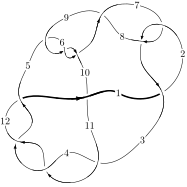
\includegraphics[width=112pt]{../../../GIT/diagram.site/Diagrams/png/1590_12a_0789.png}\\
\ \ \ A knot diagram\footnotemark}&
\allowdisplaybreaks
\textbf{Linearized knot diagam} \\
\cline{2-2}
 &
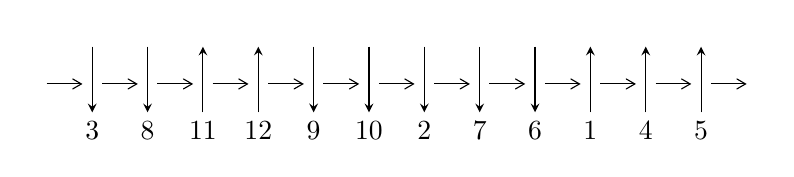
\begin{tikzpicture}[x=20pt, y=17pt]
	% nodes
	\node (C0) at (0, 0) {};
	\node (C1) at (1, 0) {};
	\node (C1U) at (1, +1) {};
	\node (C1D) at (1, -1) {3};

	\node (C2) at (2, 0) {};
	\node (C2U) at (2, +1) {};
	\node (C2D) at (2, -1) {8};

	\node (C3) at (3, 0) {};
	\node (C3U) at (3, +1) {};
	\node (C3D) at (3, -1) {11};

	\node (C4) at (4, 0) {};
	\node (C4U) at (4, +1) {};
	\node (C4D) at (4, -1) {12};

	\node (C5) at (5, 0) {};
	\node (C5U) at (5, +1) {};
	\node (C5D) at (5, -1) {9};

	\node (C6) at (6, 0) {};
	\node (C6U) at (6, +1) {};
	\node (C6D) at (6, -1) {10};

	\node (C7) at (7, 0) {};
	\node (C7U) at (7, +1) {};
	\node (C7D) at (7, -1) {2};

	\node (C8) at (8, 0) {};
	\node (C8U) at (8, +1) {};
	\node (C8D) at (8, -1) {7};

	\node (C9) at (9, 0) {};
	\node (C9U) at (9, +1) {};
	\node (C9D) at (9, -1) {6};

	\node (C10) at (10, 0) {};
	\node (C10U) at (10, +1) {};
	\node (C10D) at (10, -1) {1};

	\node (C11) at (11, 0) {};
	\node (C11U) at (11, +1) {};
	\node (C11D) at (11, -1) {4};

	\node (C12) at (12, 0) {};
	\node (C12U) at (12, +1) {};
	\node (C12D) at (12, -1) {5};
	\node (C13) at (13, 0) {};

	% arrows
	\draw[->,>={angle 60}]
	(C0) edge (C1) (C1) edge (C2) (C2) edge (C3) (C3) edge (C4) (C4) edge (C5) (C5) edge (C6) (C6) edge (C7) (C7) edge (C8) (C8) edge (C9) (C9) edge (C10) (C10) edge (C11) (C11) edge (C12) (C12) edge (C13) ;	\draw[->,>=stealth]
	(C1U) edge (C1D) (C2U) edge (C2D) (C3D) edge (C3U) (C4D) edge (C4U) (C5U) edge (C5D) (C6U) edge (C6D) (C7U) edge (C7D) (C8U) edge (C8D) (C9U) edge (C9D) (C10D) edge (C10U) (C11D) edge (C11U) (C12D) edge (C12U) ;
	\end{tikzpicture} \\
\hhline{~~} \\& 
\textbf{Solving Sequence} \\ \cline{2-2} 
 &
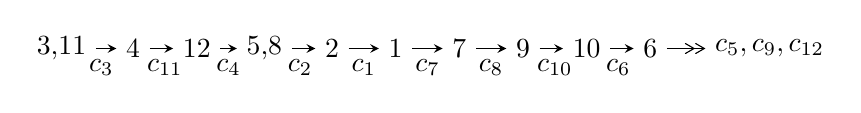
\begin{tikzpicture}[x=23pt, y=7pt]
	% node
	\node (A0) at (-1/8, 0) {3,11};
	\node (A1) at (1, 0) {4};
	\node (A2) at (2, 0) {12};
	\node (A3) at (49/16, 0) {5,8};
	\node (A4) at (33/8, 0) {2};
	\node (A5) at (41/8, 0) {1};
	\node (A6) at (49/8, 0) {7};
	\node (A7) at (57/8, 0) {9};
	\node (A8) at (65/8, 0) {10};
	\node (A9) at (73/8, 0) {6};
	\node (C1) at (1/2, -1) {$c_{3}$};
	\node (C2) at (3/2, -1) {$c_{11}$};
	\node (C3) at (5/2, -1) {$c_{4}$};
	\node (C4) at (29/8, -1) {$c_{2}$};
	\node (C5) at (37/8, -1) {$c_{1}$};
	\node (C6) at (45/8, -1) {$c_{7}$};
	\node (C7) at (53/8, -1) {$c_{8}$};
	\node (C8) at (61/8, -1) {$c_{10}$};
	\node (C9) at (69/8, -1) {$c_{6}$};
	\node (A10) at (11, 0) {$c_{5},c_{9},c_{12}$};

	% edge
	\draw[->,>=stealth]	
	(A0) edge (A1) (A1) edge (A2) (A2) edge (A3) (A3) edge (A4) (A4) edge (A5) (A5) edge (A6) (A6) edge (A7) (A7) edge (A8) (A8) edge (A9) ;
	\draw[->>,>={angle 60}]	
	(A9) edge (A10);
\end{tikzpicture} \\ 

\end{tabular} \\

\footnotetext{
The image of knot diagram is generated by the software ``\textbf{Draw programme}" developed by Andrew Bartholomew(\url{http://www.layer8.co.uk/maths/draw/index.htm\#Running-draw}), where we modified some parts for our purpose(\url{https://github.com/CATsTAILs/LinksPainter}).
}\phantom \\ \newline 
\centering \textbf{Ideals for irreducible components\footnotemark of $X_{\text{par}}$} 
 
\begin{align*}
I^u_{1}&=\langle 
- u^{55}+32 u^{53}+\cdots+b+1,\;u^{55}+u^{54}+\cdots+a-3,\;u^{56}-2 u^{55}+\cdots+4 u+1\rangle \\
I^u_{2}&=\langle 
b,\;a- u-1,\;u^2+u-1\rangle \\
\\
\end{align*}
\raggedright * 2 irreducible components of $\dim_{\mathbb{C}}=0$, with total 58 representations.\\
\footnotetext{All coefficients of polynomials are rational numbers. But the coefficients are sometimes approximated in decimal forms when there is not enough margin.}
\newpage
\renewcommand{\arraystretch}{1}
\centering \section*{I. $I^u_{1}= \langle - u^{55}+32 u^{53}+\cdots+b+1,\;u^{55}+u^{54}+\cdots+a-3,\;u^{56}-2 u^{55}+\cdots+4 u+1 \rangle$}
\flushleft \textbf{(i) Arc colorings}\\
\begin{tabular}{m{7pt} m{180pt} m{7pt} m{180pt} }
\flushright $a_{3}=$&$\begin{pmatrix}1\\0\end{pmatrix}$ \\
\flushright $a_{11}=$&$\begin{pmatrix}0\\u\end{pmatrix}$ \\
\flushright $a_{4}=$&$\begin{pmatrix}1\\- u^2\end{pmatrix}$ \\
\flushright $a_{12}=$&$\begin{pmatrix}u\\- u^3+u\end{pmatrix}$ \\
\flushright $a_{5}=$&$\begin{pmatrix}- u^2+1\\u^4-2 u^2\end{pmatrix}$ \\
\flushright $a_{8}=$&$\begin{pmatrix}- u^{55}- u^{54}+\cdots+3 u+3\\u^{55}-32 u^{53}+\cdots-6 u-1\end{pmatrix}$ \\
\flushright $a_{2}=$&$\begin{pmatrix}- u^5+2 u^3+u\\u^5-3 u^3+u\end{pmatrix}$ \\
\flushright $a_{1}=$&$\begin{pmatrix}- u^3+2 u\\u^5-3 u^3+u\end{pmatrix}$ \\
\flushright $a_{7}=$&$\begin{pmatrix}u^{55}- u^{54}+\cdots-2 u+2\\- u^{55}+32 u^{53}+\cdots+3 u+1\end{pmatrix}$ \\
\flushright $a_{9}=$&$\begin{pmatrix}- u^{55}- u^{54}+\cdots+5 u+3\\u^{55}-32 u^{53}+\cdots-6 u-1\end{pmatrix}$ \\
\flushright $a_{10}=$&$\begin{pmatrix}- u^7+4 u^5-4 u^3\\u^9-5 u^7+7 u^5-2 u^3+u\end{pmatrix}$ \\
\flushright $a_{6}=$&$\begin{pmatrix}- u^{54}+u^{53}+\cdots+2 u+3\\- u^{29}+17 u^{27}+\cdots-2 u^2- u\end{pmatrix}$\\&\end{tabular}
\flushleft \textbf{(ii) Obstruction class $= -1$}\\~\\
\flushleft \textbf{(iii) Cusp Shapes $= 4 u^{55}- u^{54}+\cdots+5 u-11$}\\~\\
\newpage\renewcommand{\arraystretch}{1}
\flushleft \textbf{(iv) u-Polynomials at the component}\newline \\
\begin{tabular}{m{50pt}|m{274pt}}
Crossings & \hspace{64pt}u-Polynomials at each crossing \\
\hline $$\begin{aligned}c_{1},c_{8}\end{aligned}$$&$\begin{aligned}
&u^{56}+15 u^{55}+\cdots+216 u+16
\end{aligned}$\\
\hline $$\begin{aligned}c_{2},c_{7}\end{aligned}$$&$\begin{aligned}
&u^{56}+u^{55}+\cdots-4 u-4
\end{aligned}$\\
\hline $$\begin{aligned}c_{3},c_{4},c_{11}\\c_{12}\end{aligned}$$&$\begin{aligned}
&u^{56}-2 u^{55}+\cdots+4 u+1
\end{aligned}$\\
\hline $$\begin{aligned}c_{5},c_{6},c_{9}\end{aligned}$$&$\begin{aligned}
&u^{56}-3 u^{55}+\cdots- u-1
\end{aligned}$\\
\hline $$\begin{aligned}c_{10}\end{aligned}$$&$\begin{aligned}
&u^{56}+18 u^{55}+\cdots+6542 u+1153
\end{aligned}$\\
\hline
\end{tabular}\\~\\
\newpage\renewcommand{\arraystretch}{1}
\flushleft \textbf{(v) Riley Polynomials at the component}\newline \\
\begin{tabular}{m{50pt}|m{274pt}}
Crossings & \hspace{64pt}Riley Polynomials at each crossing \\
\hline $$\begin{aligned}c_{1},c_{8}\end{aligned}$$&$\begin{aligned}
&y^{56}+49 y^{55}+\cdots-800 y+256
\end{aligned}$\\
\hline $$\begin{aligned}c_{2},c_{7}\end{aligned}$$&$\begin{aligned}
&y^{56}-15 y^{55}+\cdots-216 y+16
\end{aligned}$\\
\hline $$\begin{aligned}c_{3},c_{4},c_{11}\\c_{12}\end{aligned}$$&$\begin{aligned}
&y^{56}-66 y^{55}+\cdots-16 y+1
\end{aligned}$\\
\hline $$\begin{aligned}c_{5},c_{6},c_{9}\end{aligned}$$&$\begin{aligned}
&y^{56}-45 y^{55}+\cdots+29 y+1
\end{aligned}$\\
\hline $$\begin{aligned}c_{10}\end{aligned}$$&$\begin{aligned}
&y^{56}-30 y^{55}+\cdots-62348032 y+1329409
\end{aligned}$\\
\hline
\end{tabular}\\~\\
\newpage\flushleft \textbf{(vi) Complex Volumes and Cusp Shapes}
$$\begin{array}{c|c|c}  
\text{Solutions to }I^u_{1}& \I (\text{vol} + \sqrt{-1}CS) & \text{Cusp shape}\\
 \hline 
\begin{aligned}
u &= \phantom{-}0.861614 + 0.380828 I \\
a &= \phantom{-}1.202800 + 0.472116 I \\
b &= -0.915762 - 0.737386 I\end{aligned}
 & \phantom{-}2.07733 - 3.75955 I & \phantom{-0.000000 -}0. + 2.06314 I \\ \hline\begin{aligned}
u &= \phantom{-}0.861614 - 0.380828 I \\
a &= \phantom{-}1.202800 - 0.472116 I \\
b &= -0.915762 + 0.737386 I\end{aligned}
 & \phantom{-}2.07733 + 3.75955 I & \phantom{-0.000000 } 0. - 2.06314 I \\ \hline\begin{aligned}
u &= -0.776749 + 0.490571 I \\
a &= -0.50179 + 2.16195 I \\
b &= -1.024790 - 0.785571 I\end{aligned}
 & \phantom{-}1.24745 - 10.95200 I & -0.88355 + 9.10486 I \\ \hline\begin{aligned}
u &= -0.776749 - 0.490571 I \\
a &= -0.50179 - 2.16195 I \\
b &= -1.024790 + 0.785571 I\end{aligned}
 & \phantom{-}1.24745 + 10.95200 I & -0.88355 - 9.10486 I \\ \hline\begin{aligned}
u &= \phantom{-}0.917254\phantom{ +0.000000I} \\
a &= -0.937794\phantom{ +0.000000I} \\
b &= \phantom{-}0.865247\phantom{ +0.000000I}\end{aligned}
 & -2.32133\phantom{ +0.000000I} & -4.40840\phantom{ +0.000000I} \\ \hline\begin{aligned}
u &= \phantom{-}0.813380 + 0.406723 I \\
a &= -1.172270 - 0.567248 I \\
b &= \phantom{-}0.827652 + 0.819827 I\end{aligned}
 & \phantom{-}6.04894 + 0.47222 I & \phantom{-}4.63325 - 1.43874 I \\ \hline\begin{aligned}
u &= \phantom{-}0.813380 - 0.406723 I \\
a &= -1.172270 + 0.567248 I \\
b &= \phantom{-}0.827652 - 0.819827 I\end{aligned}
 & \phantom{-}6.04894 - 0.47222 I & \phantom{-}4.63325 + 1.43874 I \\ \hline\begin{aligned}
u &= -0.782454 + 0.456203 I \\
a &= \phantom{-}0.58253 - 2.23050 I \\
b &= \phantom{-}0.943810 + 0.783646 I\end{aligned}
 & \phantom{-}5.68928 - 6.47510 I & \phantom{-}3.47548 + 7.00475 I \\ \hline\begin{aligned}
u &= -0.782454 - 0.456203 I \\
a &= \phantom{-}0.58253 + 2.23050 I \\
b &= \phantom{-}0.943810 - 0.783646 I\end{aligned}
 & \phantom{-}5.68928 + 6.47510 I & \phantom{-}3.47548 - 7.00475 I \\ \hline\begin{aligned}
u &= \phantom{-}0.768228 + 0.434814 I \\
a &= \phantom{-}1.144950 + 0.658680 I \\
b &= -0.742662 - 0.902492 I\end{aligned}
 & \phantom{-}2.13106 + 4.71480 I & \phantom{-}0.47050 - 5.02848 I\\
 \hline 
 \end{array}$$\newpage$$\begin{array}{c|c|c}  
\text{Solutions to }I^u_{1}& \I (\text{vol} + \sqrt{-1}CS) & \text{Cusp shape}\\
 \hline 
\begin{aligned}
u &= \phantom{-}0.768228 - 0.434814 I \\
a &= \phantom{-}1.144950 - 0.658680 I \\
b &= -0.742662 + 0.902492 I\end{aligned}
 & \phantom{-}2.13106 - 4.71480 I & \phantom{-}0.47050 + 5.02848 I \\ \hline\begin{aligned}
u &= -0.778193 + 0.407597 I \\
a &= -0.71065 + 2.31160 I \\
b &= -0.838906 - 0.752287 I\end{aligned}
 & \phantom{-}2.31622 - 1.89869 I & \phantom{-}0.70275 + 3.94226 I \\ \hline\begin{aligned}
u &= -0.778193 - 0.407597 I \\
a &= -0.71065 - 2.31160 I \\
b &= -0.838906 + 0.752287 I\end{aligned}
 & \phantom{-}2.31622 + 1.89869 I & \phantom{-}0.70275 - 3.94226 I \\ \hline\begin{aligned}
u &= -0.570014 + 0.501355 I \\
a &= \phantom{-}0.76909 - 1.45994 I \\
b &= \phantom{-}1.087280 + 0.321819 I\end{aligned}
 & -6.02729 - 5.28844 I & -6.96026 + 7.61800 I \\ \hline\begin{aligned}
u &= -0.570014 - 0.501355 I \\
a &= \phantom{-}0.76909 + 1.45994 I \\
b &= \phantom{-}1.087280 - 0.321819 I\end{aligned}
 & -6.02729 + 5.28844 I & -6.96026 - 7.61800 I \\ \hline\begin{aligned}
u &= -0.544488 + 0.378983 I \\
a &= -1.32009 + 1.52978 I \\
b &= -0.842302 - 0.270646 I\end{aligned}
 & -0.55880 - 2.99317 I & -2.43682 + 9.49735 I \\ \hline\begin{aligned}
u &= -0.544488 - 0.378983 I \\
a &= -1.32009 - 1.52978 I \\
b &= -0.842302 + 0.270646 I\end{aligned}
 & -0.55880 + 2.99317 I & -2.43682 - 9.49735 I \\ \hline\begin{aligned}
u &= -0.079318 + 0.638620 I \\
a &= \phantom{-}0.556233 + 0.364082 I \\
b &= \phantom{-}0.992202 - 0.742680 I\end{aligned}
 & -0.82232 + 7.15155 I & -4.60706 - 5.03276 I \\ \hline\begin{aligned}
u &= -0.079318 - 0.638620 I \\
a &= \phantom{-}0.556233 - 0.364082 I \\
b &= \phantom{-}0.992202 + 0.742680 I\end{aligned}
 & -0.82232 - 7.15155 I & -4.60706 + 5.03276 I \\ \hline\begin{aligned}
u &= -0.316519 + 0.540275 I \\
a &= -0.814732 + 0.436386 I \\
b &= -1.068200 + 0.206607 I\end{aligned}
 & -6.75768 + 1.69595 I & -9.62058 - 0.39515 I\\
 \hline 
 \end{array}$$\newpage$$\begin{array}{c|c|c}  
\text{Solutions to }I^u_{1}& \I (\text{vol} + \sqrt{-1}CS) & \text{Cusp shape}\\
 \hline 
\begin{aligned}
u &= -0.316519 - 0.540275 I \\
a &= -0.814732 - 0.436386 I \\
b &= -1.068200 - 0.206607 I\end{aligned}
 & -6.75768 - 1.69595 I & -9.62058 + 0.39515 I \\ \hline\begin{aligned}
u &= \phantom{-}0.605204 + 0.139914 I \\
a &= \phantom{-}0.523878 + 0.514590 I \\
b &= -0.281922 - 0.406522 I\end{aligned}
 & \phantom{-}1.104200 + 0.351253 I & \phantom{-}7.66165 - 1.23198 I \\ \hline\begin{aligned}
u &= \phantom{-}0.605204 - 0.139914 I \\
a &= \phantom{-}0.523878 - 0.514590 I \\
b &= -0.281922 + 0.406522 I\end{aligned}
 & \phantom{-}1.104200 - 0.351253 I & \phantom{-}7.66165 + 1.23198 I \\ \hline\begin{aligned}
u &= -0.038185 + 0.607819 I \\
a &= -0.646423 - 0.466088 I \\
b &= -0.882448 + 0.766731 I\end{aligned}
 & \phantom{-}3.48917 + 2.89621 I & -0.22897 - 2.80424 I \\ \hline\begin{aligned}
u &= -0.038185 - 0.607819 I \\
a &= -0.646423 + 0.466088 I \\
b &= -0.882448 - 0.766731 I\end{aligned}
 & \phantom{-}3.48917 - 2.89621 I & -0.22897 + 2.80424 I \\ \hline\begin{aligned}
u &= \phantom{-}0.457801 + 0.362756 I \\
a &= -0.775748 - 0.907568 I \\
b &= \phantom{-}0.118428 + 0.812194 I\end{aligned}
 & -2.68266 + 1.34854 I & -4.20838 - 4.89529 I \\ \hline\begin{aligned}
u &= \phantom{-}0.457801 - 0.362756 I \\
a &= -0.775748 + 0.907568 I \\
b &= \phantom{-}0.118428 - 0.812194 I\end{aligned}
 & -2.68266 - 1.34854 I & -4.20838 + 4.89529 I \\ \hline\begin{aligned}
u &= \phantom{-}0.024733 + 0.567150 I \\
a &= \phantom{-}0.743934 + 0.615367 I \\
b &= \phantom{-}0.729699 - 0.800933 I\end{aligned}
 & -0.035156 - 1.335270 I & -3.76168 + 0.44055 I \\ \hline\begin{aligned}
u &= \phantom{-}0.024733 - 0.567150 I \\
a &= \phantom{-}0.743934 - 0.615367 I \\
b &= \phantom{-}0.729699 + 0.800933 I\end{aligned}
 & -0.035156 + 1.335270 I & -3.76168 - 0.44055 I \\ \hline\begin{aligned}
u &= \phantom{-}1.44775\phantom{ +0.000000I} \\
a &= -0.137478\phantom{ +0.000000I} \\
b &= \phantom{-}1.13818\phantom{ +0.000000I}\end{aligned}
 & -1.53547\phantom{ +0.000000I} & \phantom{-0.000000 } 0\\
 \hline 
 \end{array}$$\newpage$$\begin{array}{c|c|c}  
\text{Solutions to }I^u_{1}& \I (\text{vol} + \sqrt{-1}CS) & \text{Cusp shape}\\
 \hline 
\begin{aligned}
u &= -0.316942 + 0.333544 I \\
a &= \phantom{-}1.67144 - 0.45362 I \\
b &= \phantom{-}0.730562 - 0.086920 I\end{aligned}
 & -1.184330 + 0.293211 I & -7.24661 - 0.11134 I \\ \hline\begin{aligned}
u &= -0.316942 - 0.333544 I \\
a &= \phantom{-}1.67144 + 0.45362 I \\
b &= \phantom{-}0.730562 + 0.086920 I\end{aligned}
 & -1.184330 - 0.293211 I & -7.24661 + 0.11134 I \\ \hline\begin{aligned}
u &= -1.54283 + 0.06225 I \\
a &= \phantom{-}0.45736 - 1.45447 I \\
b &= -0.258482 + 0.942392 I\end{aligned}
 & \phantom{-}4.08661 - 2.66620 I & \phantom{-0.000000 } 0 \\ \hline\begin{aligned}
u &= -1.54283 - 0.06225 I \\
a &= \phantom{-}0.45736 + 1.45447 I \\
b &= -0.258482 - 0.942392 I\end{aligned}
 & \phantom{-}4.08661 + 2.66620 I & \phantom{-0.000000 } 0 \\ \hline\begin{aligned}
u &= \phantom{-}1.54469 + 0.03373 I \\
a &= -0.851909 - 0.654429 I \\
b &= -0.876218 + 0.153382 I\end{aligned}
 & \phantom{-}5.30389 + 0.47425 I & \phantom{-0.000000 } 0 \\ \hline\begin{aligned}
u &= \phantom{-}1.54469 - 0.03373 I \\
a &= -0.851909 + 0.654429 I \\
b &= -0.876218 - 0.153382 I\end{aligned}
 & \phantom{-}5.30389 - 0.47425 I & \phantom{-0.000000 } 0 \\ \hline\begin{aligned}
u &= \phantom{-}1.54394 + 0.12483 I \\
a &= \phantom{-}0.126116 - 1.372580 I \\
b &= -1.122220 + 0.424521 I\end{aligned}
 & \phantom{-}1.01324 + 7.50643 I & \phantom{-0.000000 } 0 \\ \hline\begin{aligned}
u &= \phantom{-}1.54394 - 0.12483 I \\
a &= \phantom{-}0.126116 + 1.372580 I \\
b &= -1.122220 - 0.424521 I\end{aligned}
 & \phantom{-}1.01324 - 7.50643 I & \phantom{-0.000000 } 0 \\ \hline\begin{aligned}
u &= \phantom{-}1.55716 + 0.08171 I \\
a &= \phantom{-}0.395590 + 1.327910 I \\
b &= \phantom{-}0.950907 - 0.362288 I\end{aligned}
 & \phantom{-}6.54610 + 4.55343 I & \phantom{-0.000000 } 0 \\ \hline\begin{aligned}
u &= \phantom{-}1.55716 - 0.08171 I \\
a &= \phantom{-}0.395590 - 1.327910 I \\
b &= \phantom{-}0.950907 + 0.362288 I\end{aligned}
 & \phantom{-}6.54610 - 4.55343 I & \phantom{-0.000000 } 0\\
 \hline 
 \end{array}$$\newpage$$\begin{array}{c|c|c}  
\text{Solutions to }I^u_{1}& \I (\text{vol} + \sqrt{-1}CS) & \text{Cusp shape}\\
 \hline 
\begin{aligned}
u &= -1.59291 + 0.03318 I \\
a &= -0.437806 + 0.931798 I \\
b &= \phantom{-}0.277160 - 0.618435 I\end{aligned}
 & \phantom{-}8.71978 - 0.96955 I & \phantom{-0.000000 } 0 \\ \hline\begin{aligned}
u &= -1.59291 - 0.03318 I \\
a &= -0.437806 - 0.931798 I \\
b &= \phantom{-}0.277160 + 0.618435 I\end{aligned}
 & \phantom{-}8.71978 + 0.96955 I & \phantom{-0.000000 } 0 \\ \hline\begin{aligned}
u &= -1.62812 + 0.12417 I \\
a &= -1.23139 + 1.34321 I \\
b &= \phantom{-}0.773399 - 0.956394 I\end{aligned}
 & \phantom{-}10.33130 - 6.82915 I & \phantom{-0.000000 } 0 \\ \hline\begin{aligned}
u &= -1.62812 - 0.12417 I \\
a &= -1.23139 - 1.34321 I \\
b &= \phantom{-}0.773399 + 0.956394 I\end{aligned}
 & \phantom{-}10.33130 + 6.82915 I & \phantom{-0.000000 } 0 \\ \hline\begin{aligned}
u &= \phantom{-}1.62976 + 0.11604 I \\
a &= \phantom{-}0.00161 + 2.29347 I \\
b &= \phantom{-}0.911680 - 0.767070 I\end{aligned}
 & \phantom{-}10.56670 + 3.88406 I & \phantom{-0.000000 } 0 \\ \hline\begin{aligned}
u &= \phantom{-}1.62976 - 0.11604 I \\
a &= \phantom{-}0.00161 - 2.29347 I \\
b &= \phantom{-}0.911680 + 0.767070 I\end{aligned}
 & \phantom{-}10.56670 - 3.88406 I & \phantom{-0.000000 } 0 \\ \hline\begin{aligned}
u &= \phantom{-}1.63214 + 0.14225 I \\
a &= -0.26342 + 2.25155 I \\
b &= \phantom{-}1.041030 - 0.821782 I\end{aligned}
 & \phantom{-}9.4693 + 13.3538 I & \phantom{-0.000000 } 0 \\ \hline\begin{aligned}
u &= \phantom{-}1.63214 - 0.14225 I \\
a &= -0.26342 - 2.25155 I \\
b &= \phantom{-}1.041030 + 0.821782 I\end{aligned}
 & \phantom{-}9.4693 - 13.3538 I & \phantom{-0.000000 } 0 \\ \hline\begin{aligned}
u &= \phantom{-}1.63313 + 0.13047 I \\
a &= \phantom{-}0.15431 - 2.28786 I \\
b &= -0.980165 + 0.809362 I\end{aligned}
 & \phantom{-}13.9539 + 8.7007 I & \phantom{-0.000000 } 0 \\ \hline\begin{aligned}
u &= \phantom{-}1.63313 - 0.13047 I \\
a &= \phantom{-}0.15431 + 2.28786 I \\
b &= -0.980165 - 0.809362 I\end{aligned}
 & \phantom{-}13.9539 - 8.7007 I & \phantom{-0.000000 } 0\\
 \hline 
 \end{array}$$\newpage$$\begin{array}{c|c|c}  
\text{Solutions to }I^u_{1}& \I (\text{vol} + \sqrt{-1}CS) & \text{Cusp shape}\\
 \hline 
\begin{aligned}
u &= -1.63993 + 0.11295 I \\
a &= \phantom{-}1.27230 - 1.22415 I \\
b &= -0.815467 + 0.876391 I\end{aligned}
 & \phantom{-}14.4734 - 2.4457 I & \phantom{-0.000000 } 0 \\ \hline\begin{aligned}
u &= -1.63993 - 0.11295 I \\
a &= \phantom{-}1.27230 + 1.22415 I \\
b &= -0.815467 - 0.876391 I\end{aligned}
 & \phantom{-}14.4734 + 2.4457 I & \phantom{-0.000000 } 0 \\ \hline\begin{aligned}
u &= -1.65226\phantom{ +0.000000I} \\
a &= \phantom{-}0.971661\phantom{ +0.000000I} \\
b &= -0.658927\phantom{ +0.000000I}\end{aligned}
 & \phantom{-}6.52621\phantom{ +0.000000I} & \phantom{-0.000000 } 0 \\ \hline\begin{aligned}
u &= -1.65143 + 0.09936 I \\
a &= -1.30952 + 1.08207 I \\
b &= \phantom{-}0.855453 - 0.778423 I\end{aligned}
 & \phantom{-}10.73980 + 1.94649 I & \phantom{-0.000000 } 0 \\ \hline\begin{aligned}
u &= -1.65143 - 0.09936 I \\
a &= -1.30952 - 1.08207 I \\
b &= \phantom{-}0.855453 + 0.778423 I\end{aligned}
 & \phantom{-}10.73980 - 1.94649 I & \phantom{-0.000000 } 0 \\ \hline\begin{aligned}
u &= -0.340130\phantom{ +0.000000I} \\
a &= \phantom{-}2.97078\phantom{ +0.000000I} \\
b &= \phantom{-}0.476062\phantom{ +0.000000I}\end{aligned}
 & -1.17659\phantom{ +0.000000I} & -11.8220\phantom{ +0.000000I}\\
 \hline 
 \end{array}$$\newpage\newpage\renewcommand{\arraystretch}{1}
\centering \section*{II. $I^u_{2}= \langle b,\;a- u-1,\;u^2+u-1 \rangle$}
\flushleft \textbf{(i) Arc colorings}\\
\begin{tabular}{m{7pt} m{180pt} m{7pt} m{180pt} }
\flushright $a_{3}=$&$\begin{pmatrix}1\\0\end{pmatrix}$ \\
\flushright $a_{11}=$&$\begin{pmatrix}0\\u\end{pmatrix}$ \\
\flushright $a_{4}=$&$\begin{pmatrix}1\\u-1\end{pmatrix}$ \\
\flushright $a_{12}=$&$\begin{pmatrix}u\\- u+1\end{pmatrix}$ \\
\flushright $a_{5}=$&$\begin{pmatrix}u\\- u\end{pmatrix}$ \\
\flushright $a_{8}=$&$\begin{pmatrix}u+1\\0\end{pmatrix}$ \\
\flushright $a_{2}=$&$\begin{pmatrix}1\\0\end{pmatrix}$ \\
\flushright $a_{1}=$&$\begin{pmatrix}1\\0\end{pmatrix}$ \\
\flushright $a_{7}=$&$\begin{pmatrix}u+1\\0\end{pmatrix}$ \\
\flushright $a_{9}=$&$\begin{pmatrix}u+1\\0\end{pmatrix}$ \\
\flushright $a_{10}=$&$\begin{pmatrix}- u\\u\end{pmatrix}$ \\
\flushright $a_{6}=$&$\begin{pmatrix}2 u+1\\- u\end{pmatrix}$\\&\end{tabular}
\flushleft \textbf{(ii) Obstruction class $= 1$}\\~\\
\flushleft \textbf{(iii) Cusp Shapes $= 5$}\\~\\
\newpage\renewcommand{\arraystretch}{1}
\flushleft \textbf{(iv) u-Polynomials at the component}\newline \\
\begin{tabular}{m{50pt}|m{274pt}}
Crossings & \hspace{64pt}u-Polynomials at each crossing \\
\hline $$\begin{aligned}c_{1},c_{2},c_{7}\\c_{8}\end{aligned}$$&$\begin{aligned}
&u^2
\end{aligned}$\\
\hline $$\begin{aligned}c_{3},c_{4}\end{aligned}$$&$\begin{aligned}
&u^2+u-1
\end{aligned}$\\
\hline $$\begin{aligned}c_{5},c_{6}\end{aligned}$$&$\begin{aligned}
&(u-1)^2
\end{aligned}$\\
\hline $$\begin{aligned}c_{9}\end{aligned}$$&$\begin{aligned}
&(u+1)^2
\end{aligned}$\\
\hline $$\begin{aligned}c_{10},c_{11},c_{12}\end{aligned}$$&$\begin{aligned}
&u^2- u-1
\end{aligned}$\\
\hline
\end{tabular}\\~\\
\newpage\renewcommand{\arraystretch}{1}
\flushleft \textbf{(v) Riley Polynomials at the component}\newline \\
\begin{tabular}{m{50pt}|m{274pt}}
Crossings & \hspace{64pt}Riley Polynomials at each crossing \\
\hline $$\begin{aligned}c_{1},c_{2},c_{7}\\c_{8}\end{aligned}$$&$\begin{aligned}
&y^2
\end{aligned}$\\
\hline $$\begin{aligned}c_{3},c_{4},c_{10}\\c_{11},c_{12}\end{aligned}$$&$\begin{aligned}
&y^2-3 y+1
\end{aligned}$\\
\hline $$\begin{aligned}c_{5},c_{6},c_{9}\end{aligned}$$&$\begin{aligned}
&(y-1)^2
\end{aligned}$\\
\hline
\end{tabular}\\~\\
\newpage\flushleft \textbf{(vi) Complex Volumes and Cusp Shapes}
$$\begin{array}{c|c|c}  
\text{Solutions to }I^u_{2}& \I (\text{vol} + \sqrt{-1}CS) & \text{Cusp shape}\\
 \hline 
\begin{aligned}
u &= \phantom{-}0.618034\phantom{ +0.000000I} \\
a &= \phantom{-}1.61803\phantom{ +0.000000I} \\
b &= \phantom{-0.000000 } 0\end{aligned}
 & -0.657974\phantom{ +0.000000I} & \phantom{-}5.00000\phantom{ +0.000000I} \\ \hline\begin{aligned}
u &= -1.61803\phantom{ +0.000000I} \\
a &= -0.618034\phantom{ +0.000000I} \\
b &= \phantom{-0.000000 } 0\end{aligned}
 & \phantom{-}7.23771\phantom{ +0.000000I} & \phantom{-}5.00000\phantom{ +0.000000I}\\
 \hline 
 \end{array}$$\newpage
\newpage\renewcommand{\arraystretch}{1}
\centering \section*{ III. u-Polynomials}
\begin{tabular}{m{50pt}|m{274pt}}
Crossings & \hspace{64pt}u-Polynomials at each crossing \\
\hline $$\begin{aligned}c_{1},c_{8}\end{aligned}$$&$\begin{aligned}
&u^2(u^{56}+15 u^{55}+\cdots+216 u+16)
\end{aligned}$\\
\hline $$\begin{aligned}c_{2},c_{7}\end{aligned}$$&$\begin{aligned}
&u^2(u^{56}+u^{55}+\cdots-4 u-4)
\end{aligned}$\\
\hline $$\begin{aligned}c_{3},c_{4}\end{aligned}$$&$\begin{aligned}
&(u^2+u-1)(u^{56}-2 u^{55}+\cdots+4 u+1)
\end{aligned}$\\
\hline $$\begin{aligned}c_{5},c_{6}\end{aligned}$$&$\begin{aligned}
&((u-1)^2)(u^{56}-3 u^{55}+\cdots- u-1)
\end{aligned}$\\
\hline $$\begin{aligned}c_{9}\end{aligned}$$&$\begin{aligned}
&((u+1)^2)(u^{56}-3 u^{55}+\cdots- u-1)
\end{aligned}$\\
\hline $$\begin{aligned}c_{10}\end{aligned}$$&$\begin{aligned}
&(u^2- u-1)(u^{56}+18 u^{55}+\cdots+6542 u+1153)
\end{aligned}$\\
\hline $$\begin{aligned}c_{11},c_{12}\end{aligned}$$&$\begin{aligned}
&(u^2- u-1)(u^{56}-2 u^{55}+\cdots+4 u+1)
\end{aligned}$\\
\hline
\end{tabular}\newpage\renewcommand{\arraystretch}{1}
\centering \section*{ IV. Riley Polynomials}
\begin{tabular}{m{50pt}|m{274pt}}
Crossings & \hspace{64pt}Riley Polynomials at each crossing \\
\hline $$\begin{aligned}c_{1},c_{8}\end{aligned}$$&$\begin{aligned}
&y^2(y^{56}+49 y^{55}+\cdots-800 y+256)
\end{aligned}$\\
\hline $$\begin{aligned}c_{2},c_{7}\end{aligned}$$&$\begin{aligned}
&y^2(y^{56}-15 y^{55}+\cdots-216 y+16)
\end{aligned}$\\
\hline $$\begin{aligned}c_{3},c_{4},c_{11}\\c_{12}\end{aligned}$$&$\begin{aligned}
&(y^2-3 y+1)(y^{56}-66 y^{55}+\cdots-16 y+1)
\end{aligned}$\\
\hline $$\begin{aligned}c_{5},c_{6},c_{9}\end{aligned}$$&$\begin{aligned}
&((y-1)^2)(y^{56}-45 y^{55}+\cdots+29 y+1)
\end{aligned}$\\
\hline $$\begin{aligned}c_{10}\end{aligned}$$&$\begin{aligned}
&(y^2-3 y+1)(y^{56}-30 y^{55}+\cdots-6.23480\times10^{7} y+1329409)
\end{aligned}$\\
\hline
\end{tabular}
\vskip 2pc
\end{document}